\documentclass{article}

\usepackage{tikz}
\usepackage{pgfplots}
\usepackage{verbatim}

\usepackage[top=1in, bottom=1.5in, left=1in, right=1in]{geometry}

\usepackage{graphicx}

\author{Stefan Seritan (PERM: 5466644), Wei Dai (CSIL: wdai, PERM: 6925747)}
\date{\today}
\title{CS140 Final Project Progress Report}

\begin{document}
\maketitle

\section*{Serial Results}
\vspace{-7pt}
\indent\indent The Metropolis Monte Carlo simulation for the Potts Lattice Gas (PLG) model was implemented in C++. The melting point and phase diagram for our test system were calculated, as shown below in Figures 1 and 2. The melting point is indicated by the peak in the heat capacity, which is at $kT = 1.35$ for this system. As for the phase diagram, the two phase region ends at $kT = 1.05$. Above this value, the solid can exist as an even mixture, while the solid will split into a species 1 rich phase and a species 2 rich phase within the two phase region (i.e. not perfect mixing). These two values will be used to ensure the algorithm remains formally correct after parallelization.

\vspace{-5pt}
\begin{center}
\textbf{Figure 1.} Heat Capacity ($\frac{dE}{dT}$) vs. Temperature ($kT$)\\
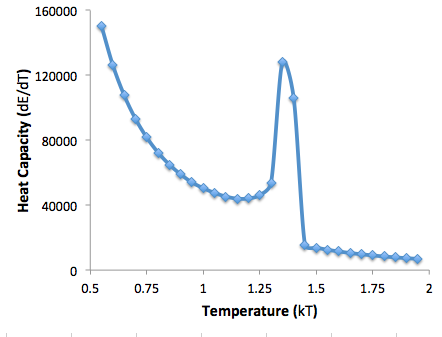
\includegraphics[scale=0.5]{SerialMeltingTemp.png}\\

\vspace{5pt}
\textbf{Figure 2.} Phase Diagram\\
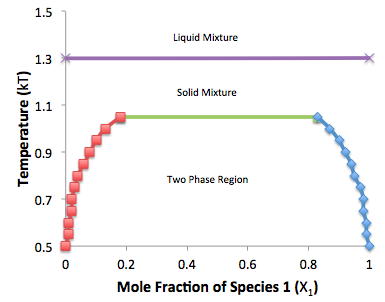
\includegraphics[scale=0.5]{SerialPhaseDiagram.png}\\
\end{center}

\newpage

\section*{Serial Performance}

\end{document}
